%% MODELO DE LATEX PARA TRABALHOS ACADÊMICOS
%% INSTRUÇÕES GERAIS:
%%    1. TODO O TEXTO NA FRENTE DO SIMBOLO '%' É COMENTÁRIO, ISTO É, ELE NÃO FAZ DIFERENÇA NO RESULTADO FINAL 
%%    2. NESTE MODELO, VOCÊS SÓ PRECISAM EDITAR DAS LINHAS 114 A 132 (INFORMAÇÕES DE CAPA) E DAS LINHAS 188 EM DIANTE (CORPO DO TRABALHO). O RESTO SÃO CONFIGURAÇÕES DE FORMATAÇÃO QUE PROVAVELMENTE NÃO SERÁ PRECISO MODIFICAR.
%%    3. MAIS INSTRUÇÕES DETALHADAS PODERÃO SER ENCONTRADAS NA PÁGINA profhelioh.wordpress.com. DÚVIDAS: heliohenrique@ufpr.br OU heliohenrique3@gmail.com

% INFORMAÇÕES DA FONTE:
%% abtex2-modelo-relatorio-tecnico.tex, v-1.7.1 laurocesar
%% Copyright 2012-2013 by abnTeX2 group at http://abntex2.googlecode.com/ 
%%
%% This work may be distributed and/or modified under the
%% conditions of the LaTeX Project Public License, either version 1.3
%% of this license or (at your option) any later version.
%% The latest version of this license is in
%%   http://www.latex-project.org/lppl.txt
%% and version 1.3 or later is part of all distributions of LaTeX
%% version 2005/12/01 or later.
%%
%% This work has the LPPL maintenance status `maintained'.
%% 
%% The Current Maintainer of this work is the abnTeX2 team, led
%% by Lauro César Araujo. Further information are available on 
%% http://abntex2.googlecode.com/
%%
%% This work consists of the files abntex2-modelo-relatorio-tecnico.tex,
%% abntex2-modelo-include-comandos and abntex2-modelo-references.bib
%%
% ------------------------------------------------------------------------
% ------------------------------------------------------------------------
% abnTeX2: Modelo de Relatório Técnico/Acadêmico em conformidade com 
% ABNT NBR 10719:2011 Informação e documentação - Relatório técnico e/ou
% científico - Apresentação
% ------------------------------------------------------------------------ 
% ------------------------------------------------------------------------

\documentclass[
	% -- opções da classe memoir --
	12pt,				% tamanho da fonte
	% openright,			% capítulos começam em pág ímpar (insere página vazia caso preciso)
    oneside,			% para impressão somente frente. Oposto a twoside (frente e verso)
	a4paper,			% tamanho do papel. 
	% -- opções da classe abntex2 --
	%chapter=TITLE,		% títulos de capítulos convertidos em letras maiúsculas
	%section=TITLE,		% títulos de seções convertidos em letras maiúsculas
	%subsection=TITLE,	% títulos de subseções convertidos em letras maiúsculas
	%subsubsection=TITLE,% títulos de subsubseções convertidos em letras maiúsculas
	% -- opções do pacote babel --
	english,			% idioma adicional para hifenização
	french,				% idioma adicional para hifenização
	spanish,			% idioma adicional para hifenização
	brazil,				% o último idioma é o principal do documento
	]{abntex2}


% ---
% PACOTES
% ---

% ---
% Pacotes fundamentais 
% ---
\usepackage{cmap}				% Mapear caracteres especiais no PDF
\usepackage{lmodern}			% Usa a fonte Latin Modern
\usepackage[T1]{fontenc}		% Selecao de codigos de fonte.
\usepackage[utf8]{inputenc}		% Codificacao do documento (conversão automática dos acentos)
\usepackage{indentfirst}		% Indenta o primeiro parágrafo de cada seção.
\usepackage{color}				% Controle das cores
\usepackage{graphicx}			% Inclusão de gráficos
% ---

% ---
% Pacotes adicionais, usados no anexo do modelo de folha de identificação
% ---
\usepackage{multicol}
\usepackage{multirow}
% ---
	
% ---
% Pacotes adicionais, usados apenas no âmbito do Modelo Canônico do abnteX2
% ---
\usepackage{lipsum}				% para geração de dummy text
% ---

% ---
% Pacotes de citações
% ---
\usepackage[brazilian,hyperpageref]{backref}	 % Paginas com as citações na bibl
\usepackage[alf]{abntex2cite}	% Citações padrão ABNT

% ---
% Pacotes de estilo
% ---
\usepackage[table,xcdraw]{xcolor}
\usepackage{array}
\usepackage{makecell}

% --- 
% CONFIGURAÇÕES DE PACOTES
% --- 

\renewcommand\theadalign{bc}
\renewcommand\theadfont{\bfseries}
\renewcommand\theadgape{\Gape[4pt]}
\renewcommand\cellgape{\Gape[4pt]}

% ---
% Configurações do pacote backref
% Usado sem a opção hyperpageref de backref
\renewcommand{\backrefpagesname}{Citado na(s) página(s):~}
% Texto padrão antes do número das páginas
\renewcommand{\backref}{}
% Define os textos da citação
\renewcommand*{\backrefalt}[4]{
	\ifcase #1 %
		Nenhuma citação no texto.%
	\or
		Citado na página #2.%
	\else
		Citado #1 vezes nas páginas #2.%
	\fi}%
% ---

% ---
% Informações de dados para CAPA e FOLHA DE ROSTO
% ---
\titulo{Apresentação de Proposta: Abordagem Genérica para Sistemas de Recomendações}
\autor{Guilherme Müller Moreira}
\orientador{Marco André Abud Kappel}
\coorientador{Luis Claudio Batista da Silva}
\local{Brasil}
\data{13 de novembro de 2018}
\instituicao{%
  Centro de Ensino Técnico Federal Celso Suckow da Fonseca
  \par
  Uned Nova Friburgo
  \par
  Sistemas de Informação}
\tipotrabalho{Relatório técnico}
% O preambulo deve conter o tipo do trabalho, o objetivo, 
% o nome da instituição e a área de concentração 
\preambulo{Apresentação da proposta de projeto para trabalho de conclusão do curso de Sistemas de Informação do CEFET Nova Friburgo. O projeto propõe uma abordagem genérica para sitemas de recomendação.}
% ---

% ---
% Configurações de aparência do PDF final

% alterando o aspecto da cor azul
\definecolor{blue}{RGB}{41,5,195}

% informações do PDF
\makeatletter
\hypersetup{
     	%pagebackref=true,
		pdftitle={\@title}, 
		pdfauthor={\@author},
    	pdfsubject={\imprimirpreambulo},
	    pdfcreator={LaTeX with abnTeX2},
		pdfkeywords={abnt}{latex}{abntex}{abntex2}{relatório técnico}, 
		colorlinks=true,       		% false: boxed links; true: colored links
    	linkcolor=blue,          	% color of internal links
    	citecolor=blue,        		% color of links to bibliography
    	filecolor=magenta,      		% color of file links
		urlcolor=blue,
		bookmarksdepth=4
}
\makeatother
% --- 

% --- 
% Espaçamentos entre linhas e parágrafos 
% --- 

% O tamanho do parágrafo é dado por:
\setlength{\parindent}{1.3cm}

% Controle do espaçamento entre um parágrafo e outro:
\setlength{\parskip}{0.2cm}  % tente também \onelineskip

% ---
% compila o indice
% ---
\makeindex
% ---

% ----
% Início do documento
% ----
\begin{document}

% Retira espaço extra obsoleto entre as frases.
\frenchspacing 

% ----------------------------------------------------------
% ELEMENTOS PRÉ-TEXTUAIS
% ----------------------------------------------------------
% \pretextual

% ---
% Capa
% ---
\imprimircapa
% ---

% ---
% Folha de rosto
% (o * indica que haverá a ficha bibliográfica)
% ---
\imprimirfolhaderosto*
% ---


% ---
% Agradecimentos
% ---
% \begin{agradecimentos}
% O agradecimento principal é direcionado a Youssef Cherem, autor do
% \nameref{formulado-identificacao} (\autopageref{formulado-identificacao}).

% Os agradecimentos especiais são direcionados ao Centro de Pesquisa em
% Arquitetura da Informação\footnote{\url{http://www.cpai.unb.br/}} da Universidade de
% Brasília (CPAI), ao grupo de usuários
% \emph{latex-br}\footnote{\url{http://groups.google.com/group/latex-br}} e aos
% novos voluntários do grupo
% \emph{\abnTeX}\footnote{\url{http://groups.google.com/group/abntex2} e
% \url{http://abntex2.googlecode.com/}}~que contribuíram e que ainda
% contribuirão para a evolução do abn\TeX.

% \end{agradecimentos}
% ---

% ---
% RESUMO
% ---

% resumo na língua vernácula (obrigatório)
\begin{resumo} %% AQUI COMEÇA A PÁGINA DE RESUMO
 FAZER

 \vspace{\onelineskip}
    
 \noindent
 \textbf{Palavras-chaves}: Recomendações. Machine Learning. 
\end{resumo} %AQUI TERMINA A PÁGINA DE RESUMO
% ---

% ---
% inserir lista de ilustrações
% ---

% \listoffigures* %% o * indica que não será incluso no sumário
\cleardoublepage %% Pula página
% ---

% ---
% inserir lista de tabelas
% ---

% \listoftables*
\cleardoublepage
% ---

% ---
% inserir lista de abreviaturas e siglas
% ---
% \begin{siglas}
%   \item[SRs] Sistemas de Recomendações
%   \item[456] Isto é um número
%   \item[123] Isto é outro número
%   \item[lauro cesar] este é o meu nome
% \end{siglas}
% ---

% ---
% inserir lista de símbolos
% ---
% \begin{simbolos}
%   \item[$ \Gamma $] Letra grega Gama
%   \item[$ \Lambda $] Lambda
%   \item[$ \zeta $] Letra grega minúscula zeta
%   \item[$ \in $] Pertence
% \end{simbolos}
% ---

% ---
% inserir o sumario
% ---

\tableofcontents*

% ---

% ----------------------------------------------------------
% ELEMENTOS TEXTUAIS  (necessário para incluir número nas páginas)
% ----------------------------------------------------------
\textual


% ----------------------------------------------------------
% Introdução
% ----------------------------------------------------------
\chapter{Introdução} %% NOVO CAPÍTULO (REPARE QUE ELE AUTOMATICAMENTE JÁ COLOCA O NÚMERO DO CAPÍTULO E JÁ ADICIONA NO SUMÁRIO)

O crescimento da internet e dos meios digitais popularizou plataformas digitais de serviços e comércio de produtos.
O número de itens nestes sistemas podem atingir quantidade e variedades grandes o suficiente para que seja difícil para o usuário 
encontrar o que busca sem o auxílio de mecanismos de filtragem. Um desses mecanismos são os sitemas de recomendação, que através de técnicas
de aprendizado de máquina e análise de dados buscam entregar conteúdo personalizado para aos usuários. Em modelos de negócio digitais a eficiência em 
oferecer informações relevantes pode ter grande impacto no sucesso do empreendimento.

Os sistemas de recomendação funcionam através da coleta de informações dos usuários ou dos elementos de um sistema, processando-as e 
identificando similaridades. Estas informações podem ser de diferentes tipos, alguns exemplos são: dados comportamentais, avaliações de usuário,
características textuais e dados audiovisuais. O processo de identificação das similaridades assim como o método de seleção das Recomendações podem 
ser implementados com diferentes abordagens. Este trabalho propõe uma abordagem genérica aos SRs utilizando técnicas de filtragem colaborativa.

Algoritmos de filtragem colaborativa funcionam organizando os usuários ou itens de um sistema em grupos com base na similaridade que possuem entre si.
Os índices de similaridade são extraídos analisando os dados de cada usuário e item do sistema. As recomendações para um usuário são geradas observando
os usuários que mais se assemelham a ele, partindo do pressuposto de que os padrões comportamentais permanecem numa tendência. 
\section{Problemas e Desafios}
A construção de um sistema de recomendações não é trivial e apresenta alguns desafios. Dentre as dificuldades recorrentes da 
implementação de SRs \citeauthoronline{2-CFSurvey} destacam:

\begin{itemize}
	\item \textbf{Esparsidade dos Dados:} Refere-se a necessidade do sistema de recomendações de lidar com itens cujos dados coletados ainda não são
	suficientes para estabelecer as similaridades com outros itens eficientemente. Este problema é comum quando um novo elemento é adicionado ao sistema. Em cenários
	como este, é improvável que o SR forneça boas recomendações.
	\item \textbf{Escalabilidade:} Conforme o número de usuários e itens de um sistema de recomendações cresce, o custo computacional para a identificação
	das similaridades pode se tornar impraticável. Com uma base de milhões de usuários e itens, um algoritmo de filtragem colaborativa com complexidade O(n)
	já se torna pesado demais \cite{2-CFSurvey}. 
	\item \textbf{Sinonímia:} Sistemas de recomendações precisam lidar com a existência de itens muito semelhantes porém com nomes ligeiramente diferentes.
	\item \textbf{Ovelhas Cinzas:} Este termo se refere aos usuários com gostos que não são suficientemente semelhantes aos de nenhum outro grupo de usuários. O sistema deve
	ser capaz de identificar este tipo de usuário de forma que ele não exerça tanta influência sobre as recomendações.
	\item \textbf{\textit{Shilling Attack}:} Neste tipo de ataque os usuários tentam manipular as recomendações parar benefício
	próprio. Isto é feito inserindo dados propositalmente no sistema, aumentando ou diminuindo a probabilidade de um item ser recomendado. É importante que existam
	mecanismos que evitem este tipo de manipulação de resultados num SR.
\end{itemize}

Os problemas acima identificados são exemplos que demonstram a não trivialidade de implementação de um SR. Além disto existem outros desafios que precisam ser
superados neste tipo de sistema, relativos a escolhas de tecnologia, arquitetura, modelagem e de abordagens técnicas. 

\section{Proposta}
Este trabalho propõe o desenvolvimento de um sistema genérico de recomendações baseado na técnica "Filtragem Colaborativa". Este sistema será utilizado como uma ferramenta
consumida por aplicações de terceiros, recebendo dados e entregando recomendações. Para satisfazer este requisito, o projeto precisa ser elaborado sobre
uma abstração que o torne independente de domínio e de tipos de cliente. A plataforma, conforme concebida, irá ser executada paralelamente às aplicações clientes,
encapsulando e solucionando os desafios inerentes aos SRs.

Outra característica importante do projeto é ser capaz de intercambear diferentes algorítmos de filtragem colaborativa, a fim de se adequar às diferentes necessidades
das aplicações clientes. Esta flexibilidade tem ainda outras motivações, que serão detalhadas ao longo deste documento. 

O sistema proposto será uma aplicação de \textit{CLI} e utilizará dois tipos de interface para se comunicar com os clientes. A primeira delas, utilizada para coleta 
de dados, será a leitura de logs de atividades gerados pela aplicação cliente e que seguem a abstração definida pela ferramenta. Esta leitura será executada em períodos 
de tempo pré configurados. Já o consumo das recomendações será feito pela segunda interface de comunicação: uma API Rest. O papel desta API, além de entregar as
recomendações é também o de permitir inserir dados específicos, descritos ao longo deste documento. 

\section{Motivações}
O desenvolvimento da ferramenta proposta possui duas principais motivações. A primeira delas, relacionada às dificuldades de se desenvolver um SR, é facilitar o uso
de recomendações em qualquer tipo de aplicação, com o menor custo de implementação possível. A ferramenta proposta permitirá que as aplicações clientes lidem apenas
com a inserção de dados e consumo das recomendações. Tornar a implementação da funcionalidade de recomendações mais trivial permitirá que sistemas de menor porte
possam oferecer este tipo de recurso.

A segunda motivação esta relacionada a capacidade de troca dos algorítmos utilizados pela ferramenta. Este recurso
permitirá a análise da eficiência dos algoritmos em diferentes cenários.

\section{Objetivos}
Os objetivos do projeto foram divididos em macro objetivos, que caracterizam os principais requisitos do projeto, e micro objetivos, que caracterizam as principais
entregas que compõem os macro objetivos.

\subsection{Macro Objetivos}
\begin{itemize}
	\item Ser capaz de coletar dados padronizados de uma fonte preenchida pelos clientes do sistema.
	\item Ser aplicável a qualquer tipo de aplicação cliente.
	\item Permitir a escolha dos seguintes componentes do sistema via configuração: Índice de Similaridade, Técnica de Cluster e o Algoritmo de Seleção das Recomendações. 
	\item Estabelecer indicadores de eficiência para diferentes configurações do item anterior e desenvolver uma análise comparatória entre elas.
\end{itemize}

\subsection{Micro Objetivos}
\begin{itemize}
	\item Estabelecer uma abstração dos elementos comuns em sistemas de recomendação.
	\item Definir uma interface de dados a ser utilizada pelo cliente ao fornecer dados para a ferramenta.
	\item Estabelecer regras de leitura dos dados fornecidos pelo cliente.
	\item Projetar o sistema de maneira modular.
	\item Implementar ao menos duas opções para cada componente cambiável do sistema.
	\item Implementar uma API Rest com autenticação para o consumo das recomendações.
\end{itemize}

\section{Estrutura do Documento}
Este documento está dividido da seguinte maneira: O capítulo "Revisão Bibliográfica" apresenta uma revisão das principais referencias da bibliografia utilizada na montagem da proposta.
Cada seção deste capítulo se refere a um artigo ou livro utilizado. Ainda neste capítulo a seção "Ferramentas Relacionadas" apresenta os resultados da pesquisa por software existentes 
que tenham objetivos semelhantes aos estabelecidos nesta proposta.

O Capítulo "Metodologia" contém detalhes a cerca do que foi planejado para a parte técnica do projeto, detalhendo e justificando as técnicas utilizadas para a construção da ferramenta
projetada.

\chapter{Revisão Bibliográfica}
Neste capítulo serão revisados os materiais utilizados como fonte de pesquisa e referência para a elaboração desta proposta. Serão analisados também softwares 
existentes no mercado e suas diferenças para a ferramenta proposta neste documento.

\section{\citeonline{1-Oreilly}}
O livro de \citeauthoronline{1-Oreilly} aborda teoria e prática de diversos tópicos relacionados a sistemas de recomendações. Dentre os temas tratados 
a Filtragem Colaborativa é definida como uma aplicação de um conceito conhecido como Inteligência Coletiva. Este termo se refere a informações que são derivadas
de um coletivo de indivíduos. No seu conceito mais básico, técnicas de CF funciona identificando usuários com característica ou gostos semelhantes entre uma base
de usuários \cite{1-Oreilly}.

Entre exemplos e definições \citeauthoronline{1-Oreilly} estabelece um fluxo básico para o processo de recomendação, decorrido em três etapas. A primeira etapa 
consiste em coletar os dados que relacionam os usuários aos itens do sistema. Estes dados representam padrões comportamentais ou perfis de interesse. A segunda
fase do processo consiste em estabelecer um índice de similaridade utilizado para agrupar os perfis de usuários. Este agrupamento é feito através do calculo de 
similaridade entre cada usuário do sistema, estabelecendo uma matriz "de-para". Com estas informações, a terceira etapa do processo consiste em identificar os
usuários mais similares e deles extrair como recomendações os itens com maior relevância. A relevância de um item pode ser calculada de diferentes maneiras.

Outro assunto abordado pelo livro é o uso de \textit{clusters} para estabelecer os grupos de usuários e extrair os indivíduos de maior semelhança. Esta técnica 
foi escolhida para o projeto como forma de persistir as relações entre usuários identificadas nas aplicações clientes.

\section{\citeonline{2-CFSurvey}}
O artigo de \citeauthoronline{2-CFSurvey} apresenta uma revisão das principais tecnologias e métodos utilizados em sistemas de recomendação. O trabalho foi
importante para introduzir os principais conceitos que cercam o tema da filtragem colaborativa. O trabalho apresenta também os principais problemas que 
que sistemas de recomendações enfrentam.

\citeauthoronline{2-CFSurvey} dividem os algoritmos de filtragem colaborativa em três grupos: Baseados em Memória, Baseados em Modelo e Híbridos. O primeiro 
tipo se caracterízam por serem simples e rápidos de implementar, considerando toda a base de dados para calcular similaridades e então oferecer recomendações.
Geralmente, esta abordagem relaciona a similaridade dos usuários com base nos dados em comum que possuem a cerca dos itens do sistema. Estes dados podem ser
avaliações, contagens de acesso etc. Das características negativas deste grupo de sistemas estão a ineficácia em lidar com dados esparços e o custo computacional
elevado derivado da escala das bases de dados. 

O segundo grupo de sistemas de recomendações, os sistemas baseados em modelo, busca superar os pontos negativos do primeiro. Esta abordagem utiliza técnicas de
análise de dados e aprendizado de máquina para montar um modelo que permita fornecer recomendações. 

Os sistemas de recomendação híbridos, categoria da ferramenta proposta neste documento, combínam características de filtragem colaborativa com filtragem baseada
em conteúdo. Neste grupo, os algoritmos utilizam os dados que coleta dos usuários em relação aos itens assim como dados das características dos itens.
combinando estes dois tipos de informações o sistema se torna mais eficiente contra a esparcidade de dados e as Ovelhas Cinzas.

O artigo estabelece uma introdução à diferentes algoritmos de cada grupo citado acima. Introduz também métricas de eficiência para SRs como
erro absoluto médio e \textit{Root Mean Squared Error}, que serão utilizadas para elaborar a análise de eficiência dos algoritimos implementados no projeto.

\section{\citeonline{5-GoogleCollaborativeFiltering}}
Este artigo apresenta uma proposta de solução para a sugestão de notícias do \textit{website} Google News. A solução precisa satisfazer dois requisitos principais:
Escalabilidade e Velocidade de Atualização do Modelo. Além disto é interessante que o algoritmo seja agnóstico e reutilizável em aplicações de diferentes domínios 
da empresa.

A solução proposta consiste em mesclar técnicas baseadas em memória e de modelo para gerar as recomendações. Da parte baseada em modelo são utilizadas duas técnicas
de \textit{cluster} - \textit{PLSI} e MinHash - enquanto que dos métdos de memória foi utilizada a \textit{item covisitation}. No modelo proposto, cada acesso a um 
\textit{link} da plataforma \textit{Google News} é registrado no histórico do usuário. O índice de similaridade dos usuários é calculado através da intersecção dos
históricos de acesso enquanto que o algorítmo \textit{PLSI} classifica os usuários em grupos e os links em gêneros.

A solução descrita no artigo de \citeonline{5-GoogleCollaborativeFiltering} se difere do projeto proposto neste documento em alguns pontos:

\begin{enumerate}
	\item \textbf{Categorização dos Itens:} No modelo proposto por \citeonline{5-GoogleCollaborativeFiltering} os itens (notícias) são categorizados conforme os acessos que recebe. Visando a solucionar
	o problema da esparsidade de dados o projeto proposto possibilita a categorização dos itens adicionados. Esta categoria terá influência nas recomendações de forma que mesmo itens recém adicionados
	possam ser recomendados.
	\item \textbf{Formato dos Dados:} Os dados utilizados na solução utilizada para a ferramenta do Google baseiam-se no histórico de acesso às notícias. A unidade escolhida foi a booleana - se um
	um usuário acessou uma notícia o valor é 1, do contrário é 0. A ferramenta descrita nesta proposta se difere em dois pontos: 1. Adota um sistema de verbos para indicar uma ação de um usuário;
	2. Contabiliza as ações dos usuários de maneira incremental. Estas diferenças permitem identificar quais itens são mais relevantes assim como qual operação sobre o item é mais relevante para o usuário.
	\item \textbf{Configuração dos Algoritmos:} A ferramenta génerica de recomendações conforme concebida se propõe a ser capaz de implementar e utilizar diferentes tipos de algorítmos de filtragem colaborativa,
	diferentemente da solução do referido artigo que se foca em apenas uma abordagem.
\end{enumerate}

\section{\citeonline{7-MeasuresBetweenSamples}}
O material acadêmico do professor e autor Michael J. Greenacre apresenta as variações dos métodos euclidianos de cálculo de distância entre amostras de dados. Os algoritmos apresentados são:

\begin{itemize}
	\item \textbf{Distância Euclidiana:} Utiliza o teorema de pitágoras para calcular a distância absoluta entre dois vetores \textit{n}-dimensionais. Este método pode ser utilizado adicionando os dados extraídos 
	dos clientes minimamente tratados como vetores para cálculo de distância. Esta distância pode ser interpretada como um índice de similaridade.
	\item \textbf{Distância Euclidiana Normalizada:} Utilizada para vetores cujas coordenadas não estão na mesma escala e precisam ser normalizadas antes do cálculo de distância. 
	\item \textbf{Distância Euclidiana em Amostras de Contagem:} Apesar de estarem na mesma escala, a natureza do item contabilizado pode significar maior frequência de ocorrência \cite{7-MeasuresBetweenSamples}. 
	Isto significa que os dados também precisam ser normalizados antes do cálculo de distância. 
\end{itemize}

\section{Ferramentas Relacionadas}
A partir de buscas na internet diferentes ferramentas com propostas a cerca de recomendações foram encontradas. Esta seção irá elencar e comparar estes softwares com o projeto proposto.

\begin{itemize}
	\item \textbf{Episerver:}\footnote{https://www.episerver.com} Enquadra-se no modelo de softwares como serviços. Possui foco em ecommerce e oferece diferentes pacotes com diferente funcionalidades. O 
	\textit{website} do produto não revela muitos detalhes, sugerindo que o Episerver é um conjunto de soluções para \textit{e-commerce} que vão além das recomendações. Estas soluções são acopladas em
	sistemas de venda digital e executam uma série de atividades. O Módulo Episerver Perform se propõe a coletar dados dos usuários, importar o catálogo de produtos e entregar recomendações diretamente
	ao usuário. Se comparado com a proposta genérica apresentada por este documento, notam-se algumas diferenças. A primeira delas está na coleta de dados, que no sistema Episerver é uma responsabilidade 
	do sistema. A ferramenta proposta aborda passivamente esta questão, apenas recebendo as informações dos sistemas clientes. Além disso, a ferramenta não é responsável por exibir as recomendações ao usuário
	e nem conhece a estrutura dos dados que recomenda. Desta maneira mantém-se a independencia do domínio, característica aparentemente não presente no software Episerver.
	\item \textbf{Strands:}\footnote{http://retail.strands.com/products/product-recommendations/} Semelhantemente ao software anterior, este produto tem foco em \textit{e-commerce} e assume o pepel de coletor
	e exibidor das recomendações. Mais uma vez, devido ao fato de ser um sistema proprietário no modelo SaS, pouca informação sobre o funcionamento da plataforma é disponibilizada. Aparentemente, scripts
	de coleta de dados comportamentais são inseridos na loja virtual para identificar os padrões de navegação dos clientes. A entrega das recomendações é feita através da inserção de widgets que exibem
	produtos préviamente importados. Se comparado com a proposta nota-se que o sistema Strands não tem a pretenção de se manter abstrato ao domínio nem de oferecer diferentes implementações de algorítmos para escolha.
	Estas características são o que distinguem o produto citado do projeto proposto.
	\item \textbf{SLI Learning Recommendations:}\footnote{https://www.sli-systems.com/solutions/product-recommendation} Semelhantemente aos outros sistemas apresentados, o \textit{SLI Learning Recomendations} 
	tem por foco \textit{e-commerces} e funciona coletando dados através da inserção de scripts de coleta de dados na loja. Este sistema difere-se em considerar questões inerentes ao domínio das vendas digitais
	para efetuar recomendações. Os itens recomendados consideram fatores como venda cruzada, aumento da média de valor dos carrinhos, etapas do processo de compra e conversão de possíveis clientes. Além disto 
	este sistema possui uma API que permite adicionar recomendações em outros elementos como emails. O projeto proposto se difere por considerar exclusivamente os padrões comportamentais dos usuários e a
	categorização dos itens para efetuar as recomendações. Outro ponto de divergência é a abstração genérica da ferramenta projetada. 
	\item \textbf{ActionML Universal Recommender:}\footnote{https://github.com/actionml/universal-recommender} O projeto \textit{Universal Recommender} se assemelha à ferramenta proposta em manter-se abstraído
	do domínio a fim de se tornar genérico. Este sistema funciona com base no conceito de eventos, ocorrencias na aplicação cliente que podem ser utilizadas como indicadores de preferência. Os eventos são
	classificados em dois tipos de acordo com uma modelagem prévia: Eventos primários e secundários. Um evento primário é o indicador de interesse mais forte na aplicação cliente e tem mais influência nas
	recomendações. Os eventos secundários podem ser quaisquer outras ações registradas no cliente que indiquem interesse do usuário. O sistema utiliza o algorítmo \textit{Correlation Cross-Ocorrence} para 
	gerar as recomendações. Das ferramentas apresentadas é a que mais se aproxima da proposta apresentada. Dentre as diferenças se destacam a necessidade de se modelar minimamente os eventos que serão inseridos
	no sistema, o consumo das recomendações, feito através de queries e não de uma API, e a abordagem híbrida utilizada. Sobre este último item, o \textit{Universal Recommeder} permite que dados dos itens sejam 
	inseridos no sistema enquanto que a ferramenta proposta permite apenas a categorização dos itens com o objetivo de melhorar a eficiência em cenários de dados esparços.
\end{itemize} 

\chapter{Metodologia}
Neste capítulo serão detalhados o planejamento para o decorrer do projeto nos seguintes assuntos: Abstração do Modelo, Técnicas e Algoritmos, Tecnologias e
Arquitetura do Sistema.

\section{Abstração do Modelo}
O desenvolvimento do projeto será baseado na construção de uma abstração que possa representar os elementos mais comuns dos sistemas de recomendações.
Esta abstração deve ser capaz de representar elementos de qualquer domínio, mantendo a capacidade de identifica-los na aplicação cliente. Destes pressupostos estabeleceu-se o seguinte protótipo de abstração:

\begin{center}
	\begin{table}[hbt]
		\caption{Descrição dos Elementos da Abstração}
		\begin{tabular}{ | c | c | c | c |}
		  \hline
			  \thead{Elemento} & \thead{Descrição} & \thead{Formato} & \thead{Escopo} \\
		  \hline
			  Ator &  \makecell{Representa algo ou alguém que \\executa atividades no cliente}  & ID Entidade + ID Elemento & Cliente  \\
		  \hline
			  Ação &  \makecell{Representa uma funcionalidade \\ou atividade que atores podem \\executar no cliente}  & ID Único & Sistema  \\
		  \hline
			  Objeto &  \makecell{Alvo de uma Ação executada \\por um Ator no cliente}  & ID Entidade + ID Elemento & Cliente  \\
		  \hline
			  Categoria &  \makecell{Permite categorizar os objetos}  & ID Único & Sistema  \\
		  \hline
		\end{tabular}
	\end{table}
\end{center}

Para todos os elementos da abstração descrita na tabela acima a ferramenta recebe um identificador, sem saber se o elemento existe ou não no cliente. Para os elementos pertencentes ao escopo dos clientes os 
identificadores são formados por dois valores, o id da entidade e o id do elemento. Esta chave composta é utilizada apenas para que o cliente identificar os itens quando consumirem as recomendações.

Os logs de atividade preenchidos pelos clientes devem conter, num formato fixo, os dados acima para representar um histórico de atividades de seus atores. Para as Categorias o sistema irá permitir o cadastro 
prévio via API. Isto será permitido para que, também através da API, seja possível informar índices de proxímidade entre categorias de objetos. Em cenários de dados esparsos, as recomendações serão feitas considerando
os itens das categorias mais próximas.

\section{Técnicas e Algoritmos}
Esta seção destina-se a detalhar os algorítmos que serão implementados no projeto assim como justificar suas ecolhas.

\subsection{Algoritmos de Similaridade}
Os dados utilizados pela ferramenta para identificar padrões comportamentais serão dados de contagem. A ferramenta irá contabilizar a quantidade de ocorrencias de cada combinação Ator x Ação x Objeto, identificando
os comportamentos mais recorrentes dos atores nos sistemas clientes. Para identificar as similaridades a partir destes dados serão implementados os algoritmos:

\begin{itemize}
	\item \textbf{Distância Euclidiana:} Calcula a distância absoluta entre dois vetores, quanto mais próximos maiores as semelhanças entre os dados. Por ser o algorítmo mais simples será utiliado como base para as comparações.
	\item \textbf{Distância Euclidiana Normalizada:} Normaliza os dados antes de efetuar o cálculo da distância. A normalização consiste em reduzir a influência das taxas de ocorrencia dos itens contabilizados, isto por que a contagem de um item
	pode ser mais alta por possuir uma taxa de ocorrencia maior que a dos outros. Outra etapa da normalizacão é efetuar o cálculo euclidiano não sobre valores absolutos, mas sobre a porcentagem de ocorrencias de um item em relação ao total de ocorrencias.
	\item \textbf{Distância Euclidiana Normalizada com Relevância:}Este algorítmo, além de efetuar as normalizações citadas no item anterior, leva em consideração o índice de relevância do objeto para o ator. Este índice varia entre 0 e 1 e é extraído a 
	partir da recorrencia do objeto no histórico do ator assim como a recorrencia da categoria do objeto em questão.
	\item \textbf{Algorítmos de Pearson}: Diferentemente da distãncia euclidiana que identifica a distância entre dois vetores, o índice de pearson índica a tendencia de variação entre duas variáveis. Quanto mais próximas e proporcionais são as flutuações 
	das variáveis, maior a similaridade entre elas. Serão implementadas cada variação da distância euclidiana citadas acima porém utilizando o índice de Pearson.
\end{itemize}

Através dos índices de similaridade a ferramenta estabelece uma matriz que contém a similaridade entre cada ator do sistema.

\subsection{Algoritmo de Clusterização}
A partir de uma matriz de similaridades entre atores é gerado um modelo de \textit{clusters} que será utilizado para persistência e para consulta dos usuários com base na proximidade. Os algorítmos escolhidos para montagem dos clusters foram: 
Clusterização Hierárquica e Clusterização em Grafos. 

Algorítmos de Clusterização Hierárquica se caracterizam por montar uma estrutura de árvore em que as folhas são os itens (Atores) e cada nível superior da hierarquia é formado por um cluster da junção dos dois nós diretamente abaixo. Nestes algorítmos a raíz da árvore é um
único cluster contendo todos os outros nós da árvore.

\begin{figure}[hbt]
	\label{Árvore de Clusters Hierárquicos}
	\caption{Árvore de Clusters Hierárquicos}
	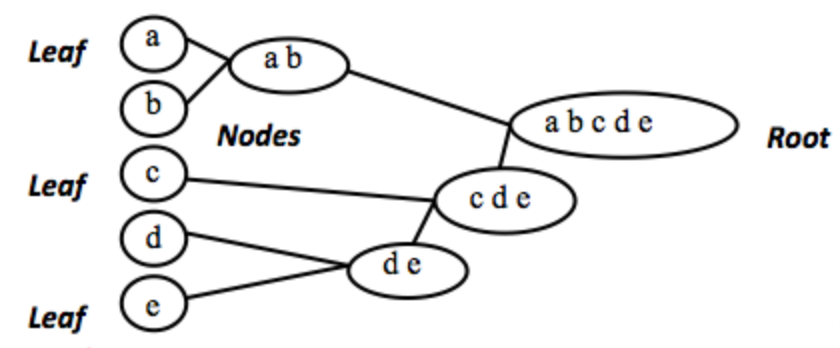
\includegraphics{hierarquical-clustering-01.png}
\end{figure}

O segundo algoritmo planejado para ser desenvolvido é o de clusterização em grafos. Neste método cada ator é representado como um nó da estrutura. Os nós mais próximos são conectados entre si com arestas que possuem pesos. Para o projeto, o peso das
arestas pode ser baseado no índice de similaridade dos atores. O grafo resultante deste método possui grupos de nós com várias conexões entre si, porém com poucas conexões com nós de outras seções. Estes grupos caracterizam os clusters.

A partir das estruturas apresentadas acima, algorítmos de seleção são utilizados para se encontrar os usuários mais próximos.

\section{Tecnologias}
Partindo dos objetivos do projeto a seguinte \textit{stack} de desenvolvimento será utilizada:

\begin{itemize}
	\item \textbf{Python:} A linguagem será utilizada para desenvolver o coletor de dados, a API Rest e os algorítmos de similaridade.
	\item \textbf{MySQL:} O SGBD será utilizado para armazenamento dos históricos comportamentais extraídos dos logs dos clientes.
	\item \textbf{Redis:} Banco de dados em memória utilizado para cache de operações em prol de performance.
	\item \textbf{Neo4J:} Base de dados para armazenamento de grafos.
	\item \textbf{Docker:} Sistema de conteiners para gerenciamento de infraestrutura.
	\item \textbf{Git:} Sistema de controle de versão do projeto.
\end{itemize}

\section{Arquitetura do Sistema}
Esta seção apresenta o protótipo inicial da arquitetura do sistema. Serão descritos os papéis de cada componente do modelo.
\begin{figure}[hbt]
	\label{Arquitetura de Componentes do Sistema}
	\caption{Arquitetura de Componentes do Sistema}
	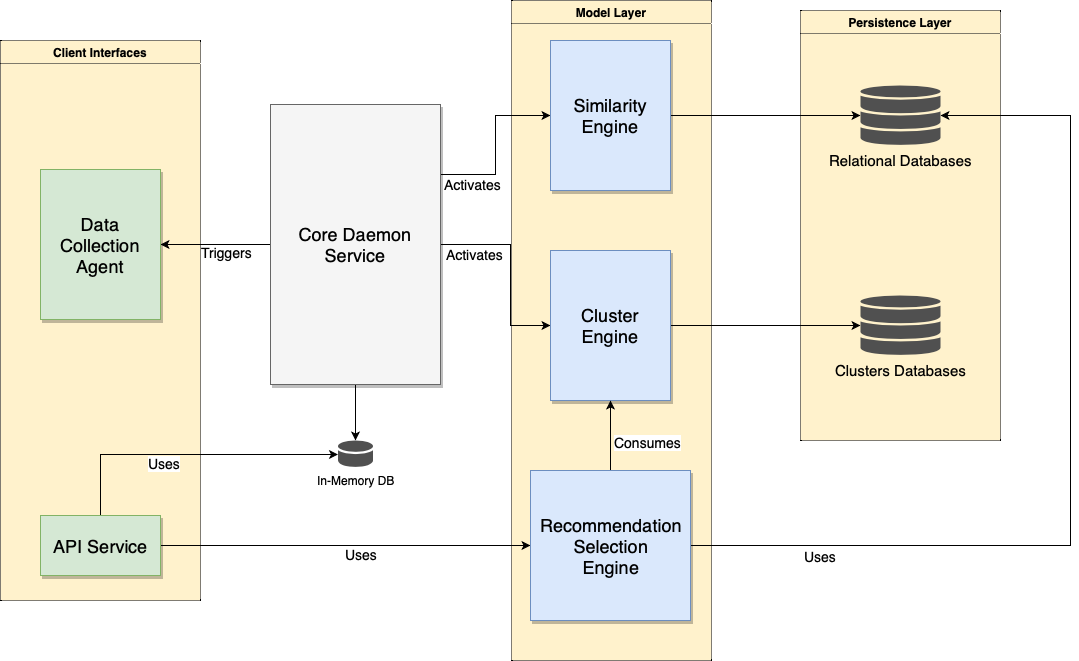
\includegraphics[width=160mm]{system-architecture.png}
\end{figure}

Na imagem acima os componentes na cor verde são os módulos e serviços que estabelecem interfaces de comunicação com as aplicações clientes. O agente de coleta de dados (\textit{Data Collection Agent}) é o módulo responsável por iterar sobre os
logs extraindo os dados. Este processo de leitura é disparado pelo núcleo do sistema (\textit{Core Service}).
O segundo elemento das interfaces de comunicação é a API que é responsável por retornar ao cliente as recomendações. A Api extrai as recomendações através do motor de seleção de recomendações. Além disto, a API também se relaciona com o banco
de dados em memória que será utilizado para disponibilizar configurações e cache de operações.

O componente central do sistema, o serviço daemon central (\textit{Core Daemon Service}), carrega a responsabilidade de manter o processo de atualização de dados em execução. Este serviço oferece ainda uma interface em CLI para configurações
de operação. Este componente dispara o agente de coleta de dados, ativa o motor de similaridade sobre os dados coletados e repassa os índices extraídos para o motor de clusterização. Assim como a API, este componente acessa a base de dados
em memória para ler e inserir configurações.

Na camada de modelo estão presentes três motores: Motor de Similaridade, Motor de Clusterização e Motor de Seleção de Recomendações. O primeiro deles é responsável por estabelecer os índices de similaridade dos atores. O segundo, de 
clusterização, recebe os dados gerados no motor de similaridade por intermédio do \textit{Core} e monta/atualiza a estrutura de clusters. Este componente é responsável ainda por extrair os atores por proximidade dos clusters. O último
motor, de seleção de recomendações, seleciona objetos e ações com base nos atores retornados pelo motor de clusters. Cada um destes motores deve ser parametrizável de maneira que seja possível escolher qual algorítmo o motor irá utilizar.

\section{Determinando Eficiência dos Algoritmos}
Visto que os componentes do sistema podem ser parametrizados de forma que utilizem diferentes algorítmos um dos objetivos deste projeto é estabelecer métricas de eficiência e comparar os algorítmos.
% TODO

\chapter{Cronograma}
A tabela abaixo apresenta o cronograma planejado para o desenvolvimento do projeto.
\begin{table}[hbt]
	\resizebox{\columnwidth}{!}{%
	\begin{tabular}{lcccccccc}
	\hline
	\multicolumn{1}{|l|}{Atividade}       & \multicolumn{1}{l|}{Mar} & \multicolumn{1}{l|}{Abr} & \multicolumn{1}{l|}{Mai} & \multicolumn{1}{l|}{Jun} & \multicolumn{1}{l|}{Jul} & \multicolumn{1}{l|}{Set} & \multicolumn{1}{l|}{Out} & \multicolumn{1}{l|}{Nov} \\ \hline
	Documentação de Requisitos            & X                        &                          &                          &                          &                          &                          &                          &                          \\
	Modelagem do Sistema                  & X                        & X                        &                          &                          &                          &                          &                          &                          \\
	Desenvolver Agente de Coleta de Dados &                          & X                        &                          &                          &                          &                          &                          &                          \\
	Desenvolver Núcleo da Aplicação       &                          &                          & X                        &                          &                          &                          &                          &                          \\
	Desenvolver Motor de Similaridade     &                          &                          & X                        & X                        &                          &                          &                          &                          \\
	Desenvolver Motor de Cluster          &                          &                          &                          & X                        & X                        &                          &                          &                          \\
	Desenvolver Motor de Coleta de Recom. &                          &                          &                          &                          &                          & X                        &                          &                          \\
	Coletar Dados de Eficiência           &                          &                          &                          &                          &                          &                          & X                        &                          \\
	Documentação e Monografia             & X                        & X                        & X                        & X                        & X                        & X                        & X                        & X                       
	\end{tabular}%
	}
\end{table} 

% A expressão \textit{\textbf{``Modelo canônico''}} é utilizada para indicar que \abnTeX\ não é
% modelo específico de nenhuma universidade ou instituição, mas que implementa tão
% somente os requisitos das normas da ABNT. Uma lista completa das normas
% observadas pelo \abnTeX\ é apresentada em \citeonline{abntex2classe}. %% USE \citeonline PARA CITAR NO MEIO DA FRASE

% \begin{figure} [hbt] 
% %% hbt SIGNIFICA QUE ELE PRIMEIRO VAI TENTAR COLOCAR A IMAGEM NESTE LUGAR (h de "here"). SENÃO DER, ELE TENTA COLOCAR MAIS PRA BAIXO (b de "bottom"). SENÃO ELE COLOCA MAIS PARA CIMA (t de "top").
% \label{figura1} 
% %% LABEL SERVE PARA VOCÊ REFERENCIAR A FIGURA NO MEIO DO TEXTO (VEJA LINHA 330: \ref{figura1}). ASSIM VOCÊ NÃO PERDE A REFERÊNCIA QUANDO MUDA A FIGURA DE LUGAR
% \caption{Exemplo de figura.}
% 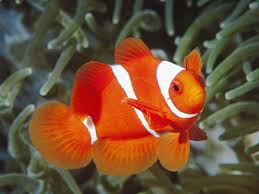
\includegraphics[width=0.95\textwidth]{nemo.jpeg} %% PARA COLOCAR O ARQUIVO DA IMAGEM NO SHARELATEX, CLIQUE NO ÍCONE QUE PARECE UMA FLECHINHA PARA CIMA (ATUALIZAR), CLIQUE EM UPLOAD E PROCURE A IMAGEM EM SEU COMPUTADOR.
% \end{figure}


% Sinta-se convidado a participar do projeto \abnTeX! Acesse o site do projeto em
% \url{http://abntex2.googlecode.com/} (Figura \ref{figura1}). Também fique livre para conhecer,
% estudar, alterar e redistribuir o trabalho do \abnTeX, desde que os arquivos
% modificados tenham seus nomes alterados e que os créditos sejam dados aos
% autores originais, nos termos da ``The \LaTeX\ Project Public
% License''\footnote{\url{http://www.latex-project.org/lppl.txt}}.

% Encorajamos que sejam realizadas customizações específicas deste exemplo para
% universidades e outras instituições --- como capas, folhas de rosto, etc.
% Porém, recomendamos que ao invés de se alterar diretamente os arquivos do
% \abnTeX, distribua-se arquivos com as respectivas customizações.
% Isso permite que futuras versões do \abnTeX~não se tornem automaticamente
% incompatíveis com as customizações promovidas. Consulte
% \citeonline{abntex2-wiki-como-customizar} par mais informações.

% Este documento deve ser utilizado como complemento dos manuais do \abnTeX\ 
% \cite{abntex2classe,abntex2cite,abntex2cite-alf} e da classe \textsf{memoir}
% \cite{memoir}. 

% Equipe \abnTeX 

% Lauro César Araujo


% ---
% Capitulo de revisão de literatura
% ---
% \chapter{Lorem ipsum dolor sit amet}

% --- Seção dentro do capítulo
% \section{Aliquam vestibulum fringilla lorem}
% ---

% \lipsum[1]  %% COMANDO QUE COLOCA TEXTO AUTOMÁTICO, SUBSTITUA POR SEU PRÓPRIO TEXTO

% \lipsum[2-3]



% ---
% Conclusão
% ---
% \chapter*[Conclusão]{Conclusão}
\addcontentsline{toc}{chapter}{Conclusão}

% \lipsum[31-33]


% ----------------------------------------------------------
% ELEMENTOS PÓS-TEXTUAIS
% ----------------------------------------------------------
\postextual


% ----------------------------------------------------------
% Referências bibliográficas
% ----------------------------------------------------------
\bibliography{abntex2-modelo-references} %% REFERENCIA AO ARQUIVO abntex2-modelo-references.bib

% ----------------------------------------------------------
% Glossário
% ----------------------------------------------------------
%
% Consulte o manual da classe abntex2 para orientações sobre o glossário.
%
%\glossary

% ----------------------------------------------------------
% Apêndices
% ----------------------------------------------------------

% ---
% Inicia os apêndices
% ---
% \begin{apendicesenv}

% Imprime uma página indicando o início dos apêndices
% \partapendices

% ----------------------------------------------------------
% \chapter{Quisque libero justo}
% ----------------------------------------------------------

% \lipsum[50]

% ----------------------------------------------------------
% \chapter{Nullam elementum urna vel imperdiet sodales elit ipsum pharetra ligula
% ac pretium ante justo a nulla curabitur tristique arcu eu metus}
% ----------------------------------------------------------
% \lipsum[55-57]

% \end{apendicesenv}
% ---


% ----------------------------------------------------------
% Anexos
% ----------------------------------------------------------

% ---
% Inicia os anexos
% ---
% \begin{anexosenv}

% % Imprime uma página indicando o início dos anexos
% \partanexos

% % ---
% \chapter{Morbi ultrices rutrum lorem.}
% % ---
% \lipsum[30]

% % ---
% \chapter{Cras non urna sed feugiat cum sociis natoque penatibus et magnis dis
% parturient montes nascetur ridiculus mus}
% % ---

% \lipsum[31]

% % ---
% \chapter{Fusce facilisis lacinia dui}
% % ---

% \lipsum[32]

% \end{anexosenv}

%---------------------------------------------------------------------
% INDICE REMISSIVO
%---------------------------------------------------------------------

\printindex

%---------------------------------------------------------------------
% Formulário de Identificação (opcional)
%---------------------------------------------------------------------
% \chapter*[Formulário de Identificação]{Formulário de Identificação}
% \addcontentsline{toc}{chapter}{Exemplo de Formulário de Identificação}
% \label{formulado-identificacao}

% Exemplo de Formulário de Identificação, compatível com o Anexo A (informativo)
% da ABNT NBR 10719:2011. Este formulário não é um anexo. Conforme definido na
% norma, ele é o último elemento pós-textual e opcional do relatório.

% \bigskip

% \begin{tabular}{|p{9cm}|p{5cm}|} %% EXEMPLO DE TABELA MAIS COMPLEXA
% \hline
% \multicolumn{2}{|c|}{\textbf{\large Dados do Relatório Técnico e/ou científico}}\\
% \hline
% \multirow{4}{10cm}[24pt]{Título e subtítulo}& Classificação de segurança\\
%                    & \\
%                    \cline{2-2}
%                    & No.\\
%                    & \\
				
% \hline
% Tipo de relatório & Data\\
% \hline
% Título do projeto/programa/plano & No.\\
% \hline
% \multicolumn{2}{|l|}{Autor(es)} \\
% \hline
% \multicolumn{2}{|l|}{Instituição executora e endereço completo} \\
% \hline
% \multicolumn{2}{|l|}{Instituição patrocinadora e endereço completo} \\
% \hline
% \multicolumn{2}{|l|}{Resumo}\\[3cm]
% \hline
% \multicolumn{2}{|l|}{Palavras-chave/descritores}\\
% \hline
% \multicolumn{2}{|l|}{
% Edição \hfill No. de páginas \hfill No. do volume \hfill Nº de classificação \phantom{XXXX}} \\
% \hline
% \multicolumn{2}{|l|}{
% ISSN \hfill \hfill Tiragem \hfill Preço \phantom{XXXXXXXX}} \\
% \hline
% \multicolumn{2}{|l|}{Distribuidor} \\
% \hline
% \multicolumn{2}{|l|}{Observações/notas}\\[3cm]
% \hline
% \end{tabular}

\end{document}
